\subsection{Vector Representations for API Usages}

\begin{figure*}[t]
\begin{center}
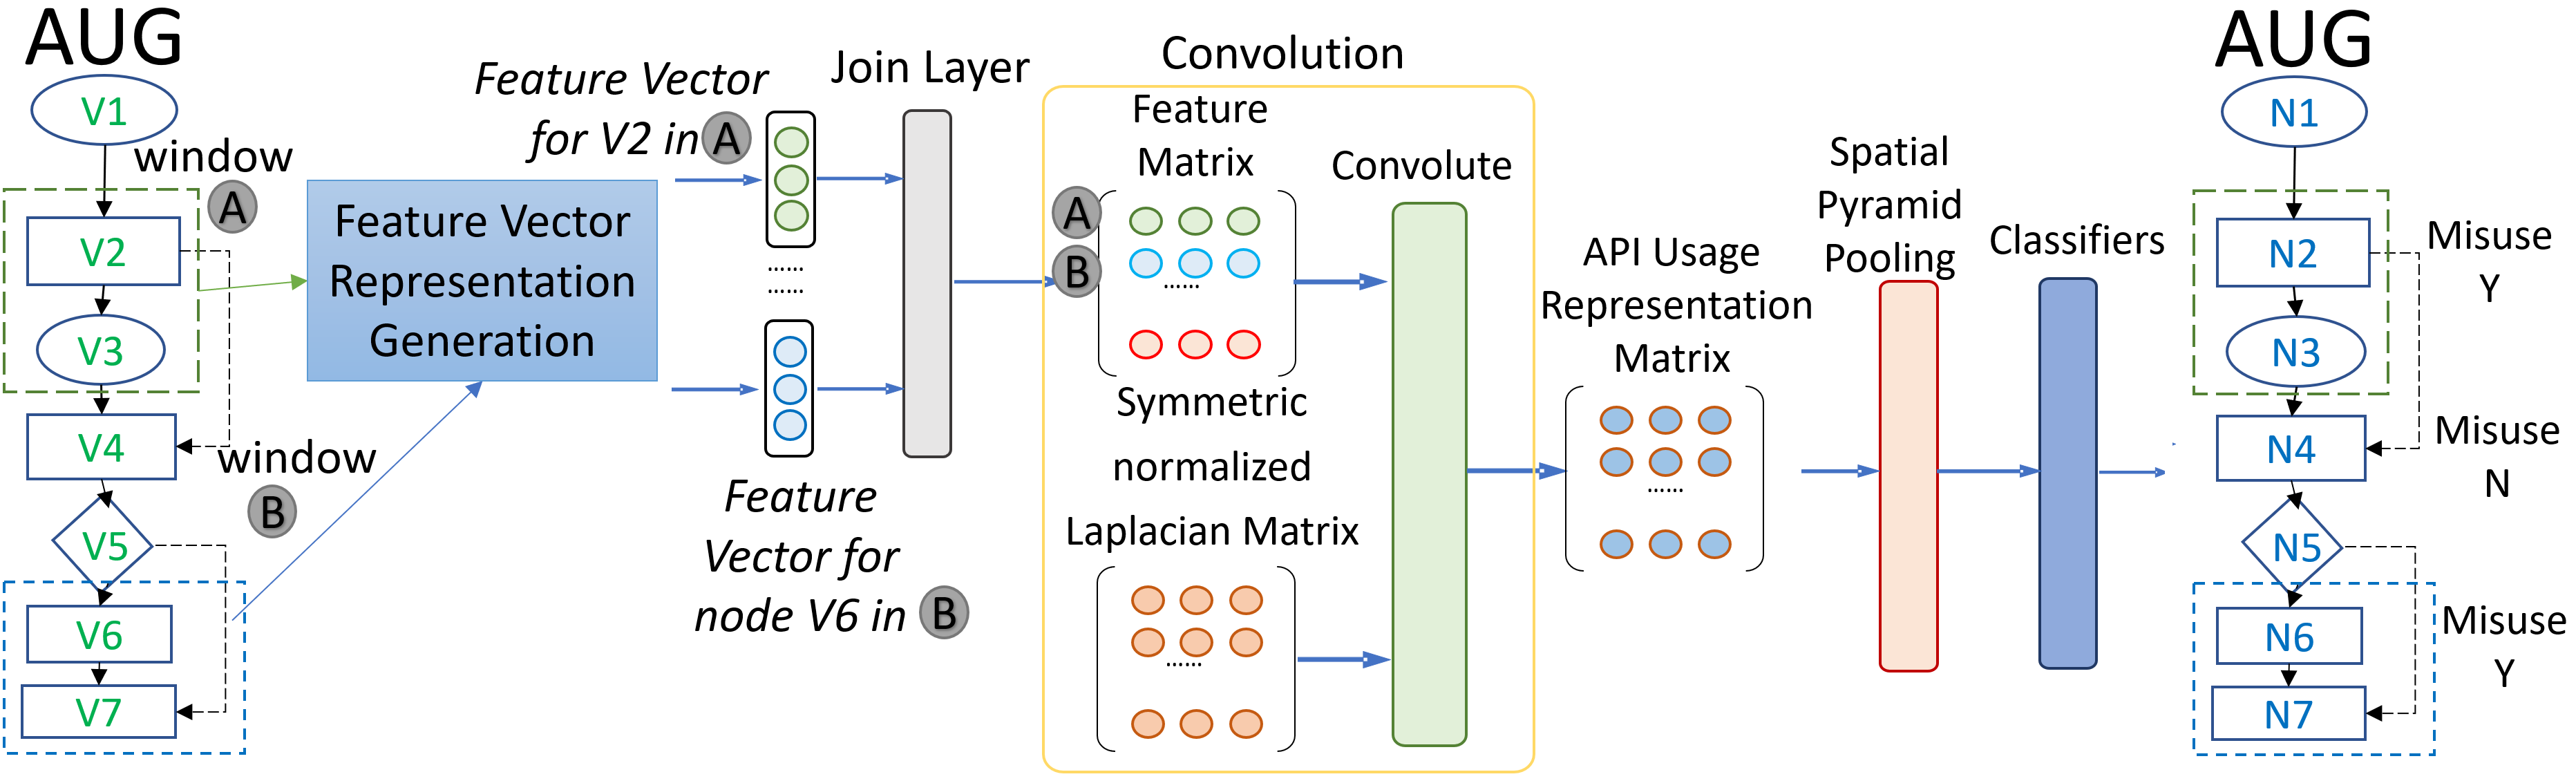
\includegraphics[width=5.6in]{gcn-detection.png}
\vspace{-5pt}
\caption{API Misuse Detection with Label-GCN}
\label{fig:gcn-detection}
\end{center}
\end{figure*}

Fig.~\ref{fig:gcn-detection} presents how we use Labelled,
Graph-based, Convolutional Network (Label-GCN)~\cite{label-gcn} to
build the vector representation (embedding) for an API usage, and then
use the learned vector for API misuse detection.

First, we parse a given method $M$ into an API usage graph. Similar to
CNN using the filter on an image, Label-GCN performs sliding a small
window along all the nodes (statements) of the PDG. For example, in
Figure~\ref{fig:gcn}, the window marked with \circled{A} for the node
$S27$ consists of itself and the neighboring statements/nodes $S6$,
$S22$, $S25$, and $S29$. Another window (marked with \circled{B}) is
for the node $S23$, including itself and the neighboring nodes: $S22$
and $S25$. For each window, FA-GCN generates the feature
representation matrix for the statement at the center. For example,
for the window centered at $S27$, it generates the feature vector
$F_{S27}$ for $S27$, using the process explained in
Figure~\ref{fig:feature}. From the representation vectors for all
statements, FA-GCN uses a join layer to link all these vectors into
the Feature Matrix $\mathcal{F}_{m}$ for method $M$. A row in
$\mathcal{F}_m$ corresponds to a window in~PDG.

Next, FA-GCN performs the convolution operation by first calculating
the symmetric normalized Laplacian matrix~$\tilde{A}$~\cite{GCN16},
and then calculating the convolution to generate the representation
matrix $M_{m}$ for the method $m$. After that, we use the traditional
steps as in a CNN model: using a spatial pyramid pooling layer (to
normalize the method representation matrix into a uniform size, and
reduce its total size), and connecting its output to a fully connected
layer to transform the matrix into a vector $V_m$ to represent
$m$. With $V_m$, we perform classification by using two hidden layers
(controlling the length of vectors and output) and a softmax function
to produce a prediction score for $m$. We use those scores as {\em
  vulnerability scores to rank the methods} in a project. The decision
for $m$ as $\mathcal{V}$ or $\mathcal{NV}$ is done via a trainable
threshold on the prediction score~\cite{li2018vuldeepecker,li2019improving}.


\subsection{Neural API Misuse Detection}

%labeling of each node in the training process: voice 1

